\documentclass{exam}

\usepackage{titling}
\usepackage{amsmath}
\usepackage{amsfonts}
\usepackage{mathtools}
\usepackage{float}
\usepackage{tikz}
\usepackage{graphicx}
\usepackage{subfig}
\usepackage{minted}
\usepackage{inconsolata}
\usepackage{tikz}
\usepackage[font={small}]{caption}

\graphicspath{ {./src/output} }

\setlength{\droptitle}{-5em}   

\renewcommand{\questionlabel}{\textbf{~\thequestion)}}
\renewcommand{\subpartlabel}{\thesubpart)}
\DeclarePairedDelimiterX{\norm}[1]{\lVert}{\rVert}{#1}

\newcommand*{\horzbar}{\rule[.5ex]{2.5ex}{0.5pt}}

\newenvironment{shiftedflalign*}{%
    \start@align\tw@\st@rredtrue\m@ne
    \hskip\parindent
}{%
    \endalign
}


\title{Homework 4 - Group 076}
\author{Aprendizagem 2021/2022}
\date{}

\cfoot{\thepage}

\begin{document}
    \maketitle
    \begin{tikzpicture}[overlay, remember picture]
        \node[xshift=3.5cm,yshift=-2cm] at (current page.north west) {
\includegraphics[scale = 0.35]{logo_ist.jpeg}};
    \end{tikzpicture}
    \vspace{-4.5em}
    \section{Pen and Paper}
    \begin{questions}
        \item Let $\textbf{c}$ be a 2-dimensional random vector for which $c_k \in \{0,1\}$ is an indicator of cluster $k$ ($k \in \{1, 2\}$ and $\sum c_k = 1$). Let $\pi_k = p(c_k = 1)$ and let $\gamma(c_{nk}) = p(c_k = 1|\textbf{x}^{(n)})$.
        \begin{itemize}
            \item \textbf{E-step} \\[0.4em]
            In this step, we assign each instance $\textbf{x}^{(n)}$ to the cluster $c_k$ that yields the largest posterior $\gamma(c_{nk})$. Given that $\textbf{x}^{(n)}|c_k = 1 \sim \mathcal{N}(\mu_k, \Sigma_k)$, by Bayes rule, we have:
            \[
                \gamma(c_{nk}) = p(c_k = 1|\textbf{x}^{(n)}) = \frac{p(c_k = 1)p(\textbf{x}^{(n)}|c_k = 1)}{\sum_{l = 1}^{2}p(c_l = 1)p(\textbf{x}^{(n)}|c_l = 1)} = \frac{\pi_k\mathcal{N}(\textbf{x}^{(n)}|\mu_k, \Sigma_k)}{\sum_{l = 1}^{2}\pi_l\mathcal{N}(\textbf{x}^{(n)}|\mu_l, \Sigma_l)}
            \]
            Setting $\mu_k = \textbf{x}^{(k)}$ ($k \in \{1, 2\})$, we now compute the posteriors:
            \begin{itemize}
                \item For $\textbf{x}^{(1)}$:
                \begin{flalign*}
                    &\gamma(c_{11}) = \frac{\pi_1\mathcal{N}(\textbf{x}^{(1)}|\mu_1, \Sigma_1)}{\sum_{l = 1}^{2}\pi_l\mathcal{N}(\textbf{x}^{(1)}|\mu_l, \Sigma_l)} = \frac{0.7 \cdot 0.1591549}{0.7 \cdot 0.1591549 + 0.3 \cdot 0.0} = \frac{0.11141}{0.11141} = 1.0 \\
                    &\gamma(c_{12}) = 1 - \gamma(c_{11}) = 0.0
                \end{flalign*}
                \item For $\textbf{x}^{(2)}$:
                \begin{flalign*}
                    \gamma(c_{21}) &= \frac{0.7 \cdot 0.0}{0.7 \cdot 0.0 +  0.3 \cdot 0.0795775} = 0.0 \quad 
                    \gamma(c_{22}) = 1 - \gamma(c_{21}) = 1.0
                \end{flalign*}
                \item For $\textbf{x}^{(3)}$:
                \begin{flalign*}
                    \hspace*{-2.1em}
                    \gamma(c_{31}) = \frac{0.7 \cdot 0.0002393}{0.7 \cdot 0.0002393 +  0.3 \cdot 0.0000098} = 0.98271 \quad  
                    \gamma(c_{32}) = 1 - \gamma(c_{31}) = 0.01729
                \end{flalign*}
                \item For $\textbf{x}^{(4)}$:
                \begin{flalign*}
                    \gamma(c_{41}) = \frac{0.7 \cdot 0.0000072}{0.7 \cdot 0.0000072 +  0.3 \cdot 0.0000028} = 0.85698 \quad  
                    \gamma(c_{42}) = 1 - \gamma(c_{41}) = 0.14302  \\
                \end{flalign*}
            \end{itemize}
            \item \textbf{M-step} \\[0.4em]
            We re-compute $\mu_k$, $\Sigma_k$ and $\pi_k$ ($k \in \{1, 2\})$ so as to increase the likelihood of the data. \\
            The new cluster centroids are given by: 
            \[
                \mu_k = \frac{\sum_{n = 1}^{4}\gamma(c_{nk})\textbf{x}^{(n)}}{\sum_{n = 1}^{4}\gamma(c_{nk})}
            \]
            And so we have:
            \[
                \mu_1 = \frac{1.0
                \begin{bmatrix}
                    2 \\ 4
                \end{bmatrix} + 0.0
                \begin{bmatrix}
                    -1 \\ -4
                \end{bmatrix} + 0.98271
                \begin{bmatrix}
                    -1 \\ 2
                \end{bmatrix} + 0.85698
                \begin{bmatrix}
                    4 \\ 0
                \end{bmatrix}
                }{1.0 + 0.0 + 0.98271 + 0.85698} = 
                \begin{bmatrix}
                    1.56538 \\
                    2.10073 \\
                \end{bmatrix}
            \]
            \[
                \mu_2 = \frac{0.0
                \begin{bmatrix}
                    2 \\ 4
                \end{bmatrix} + 1.0
                \begin{bmatrix}
                    -1 \\ -4
                \end{bmatrix} + 0.01729
                \begin{bmatrix}
                    -1 \\ 2
                \end{bmatrix} + 0.14302
                \begin{bmatrix}
                    4 \\ 0
                \end{bmatrix}
                }{0.0 + 1.0 + 0.01729 + 0.14302} = 
                \begin{bmatrix}
                    -0.3837 \\
                    -3.41758 \\
                \end{bmatrix}
            \]
            \\
            The new covariance matrices are now given by:
            \[
                \Sigma_k = \frac{\sum_{n = 1}^{4}\gamma(c_{nk})(\textbf{x}^{(n)} - \mu_k)(\textbf{x}^{(n)} - \mu_k)^T}{\sum_{n = 1}^{4}\gamma(c_{nk})}
            \]
            And so:
            \begin{align*}
                \Sigma_1 &= \frac{1.0
                \begin{bmatrix}
                    4.0 & 8.0 \\
                    8.0 & 16.0 \\
                \end{bmatrix} + 0.0
                \begin{bmatrix}
                    1.0 & 4.0 \\
                    4.0 & 16.0 \\
                \end{bmatrix} + 0.98271
                \begin{bmatrix}
                    1.0 & -2.0 \\
                    -2.0 & 4.0 \\
                \end{bmatrix} + 0.85698
                \begin{bmatrix}
                    4.0 & 0.0 \\
                    0.0 & 0.0 \\
                \end{bmatrix}
                }{1.0 + 0.0 + 0.98271 + 0.85698} = 
                \begin{bmatrix}
                    4.13282 & -1.16337 \\
                    -1.16337 & 2.6056 \\
                \end{bmatrix}\\
                \Sigma_2 &= \frac{0.0
                \begin{bmatrix}
                    4.0 & 8.0 \\
                    8.0 & 16.0 \\
                \end{bmatrix} + 1.0
                \begin{bmatrix}
                    1.0 & 4.0 \\
                    4.0 & 16.0 \\
                \end{bmatrix} + 0.01729
                \begin{bmatrix}
                    1.0 & -2.0 \\
                    -2.0 & 4.0 \\
                \end{bmatrix} + 0.14302
                \begin{bmatrix}
                    4.0 & 0.0 \\
                    0.0 & 0.0 \\
                \end{bmatrix}
                }{0.0 + 1.0 + 0.01729 + 0.14302} = 
                \begin{bmatrix}
                    2.70166 & 2.10624 \\
                    2.10624 & 2.16924 \\
                \end{bmatrix}
            \end{align*}
            Finally, the new prior probabilities can now be written as:
            \[
                \pi_k = \frac{\sum_{n = 1}^{4}\gamma(c_{nk})}{4}
            \] 
            and thus:
            \begin{align*}
                \pi_1 &= \frac{1.0 + 0.0 + 0.98271 + 0.85698}{4} = 0.70992 \\
                \pi_2 &= \frac{0.0 + 1.0 + 0.01729 + 0.14302}{4} = 0.29008 \\
            \end{align*}
            Hence, this iteration of the EM algorithm assigned points $\textbf{x}^{(1)}$, $\textbf{x}^{(3)}$ and $\textbf{x}^{(4)}$ to cluster $c_1$, while $\textbf{x}^{(2)}$ was assigned to cluster $c_2$. The following figure depicts this clustering:
            \begin{figure}[H]
                \centering
                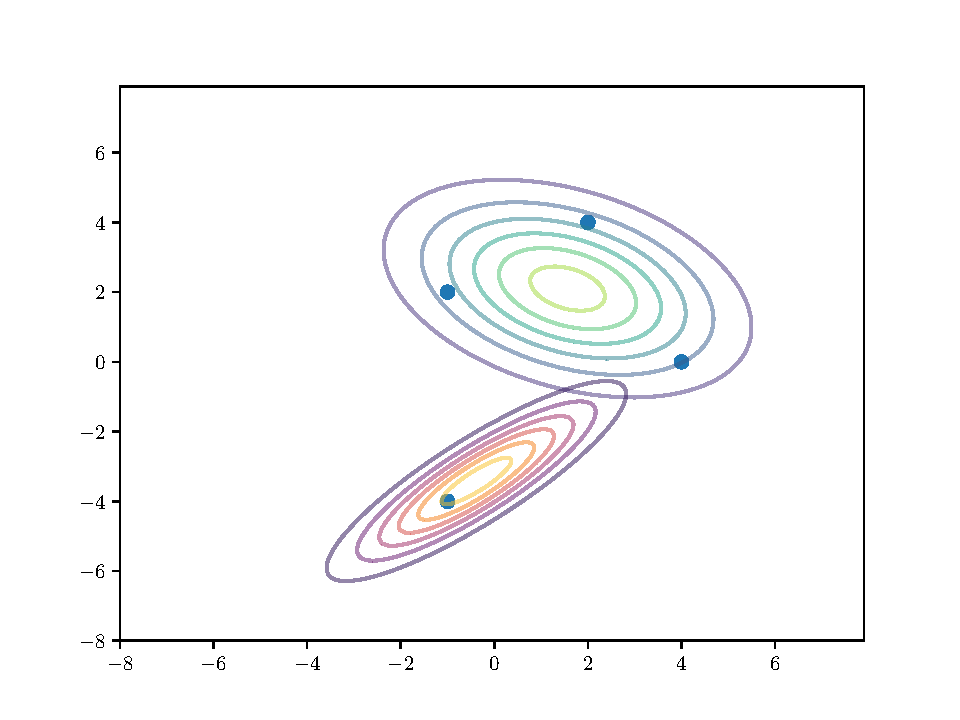
\includegraphics[scale = 0.75]{EM_clusters.pdf}
            \end{figure}
        \end{itemize}
        \item First, we compute the silhouette of cluster $c_1$:
            \begin{align*}
                s(\textbf{x}^{(1)}) &= 1 - \frac{a(\textbf{x}^{(1)})}{b(\textbf{x}^{(1)})} = 1 - \frac{\frac{\|\textbf{x}^{(1)} - \textbf{x}^{(3)}\|_2 + \|\textbf{x}^{(1)} - \textbf{x}^{(4)}\|_2}{2}}{\|\textbf{x}^{(1)} - \textbf{x}^{(2)}\|_2} = 1 - \frac{\frac{ 3.60555 + 4.47214}{2}}{8.544} = 0.52729 \\
                s(\textbf{x}^{(3)}) &= 1 - \frac{a(\textbf{x}^{(3)})}{b(\textbf{x}^{(3)})} = 1 - \frac{\frac{\|\textbf{x}^{(3)} - \textbf{x}^{(1)}\|_2 + \|\textbf{x}^{(3)} - \textbf{x}^{(4)}\|_2}{2}}{\|\textbf{x}^{(3)} - \textbf{x}^{(2)}\|_2} = 1 - \frac{\frac{ 3.60555 + 5.38516}{2}}{6.0} = 0.25077 \\
                s(\textbf{x}^{(4)}) &= 1 - \frac{a(\textbf{x}^{(4)})}{b(\textbf{x}^{(4)})} = 1 - \frac{\frac{\|\textbf{x}^{(4)} - \textbf{x}^{(1)}\|_2 + \|\textbf{x}^{(4)} - \textbf{x}^{(3)}\|_2}{2}}{\|\textbf{x}^{(4)} - \textbf{x}^{(2)}\|_2} = 1 - \frac{\frac{4.47214 + 5.38516}{2}}{6.40312} = 0.23027 \\
            \end{align*}
            \vspace{-2.2em}
            \[
                s(c_1) = \frac{ s(\textbf{x}^{(1)}) +  s(\textbf{x}^{(3)}) +  s(\textbf{x}^{(4)})}{3} = \frac{0.52729 + 0.25077 + 0.23027}{3} = 0.33611
            \]
            Since $|c_2| = 1$, we set $s(c_2) = 1$. The  silhouette of the solution is defined as the arithmetic mean of the silhouettes of the clusters:
            \vspace{1em}
            \[
                s(C) = \frac{s(c_1) + s(c_2)}{2} = \frac{0.33611 + 1.0}{2} = 0.66806
            \]
        \item \quad
        \begin{parts}
            \item \vspace{-1.6em}
            \begin{subparts}
                \item The specified MLP is described by the following parameters: weight matrices $W^{[1]}$, $W^{[2]}$, $W^{[3]}$ and $W^{[4]}$, along with bias vectors $b^{[1]}$, $b^{[2]}$, $b^{[3]}$ and $b^{[4]}$. For input data of dimention $d$, we have:
                \begin{itemize}
                    \vspace{0.6em}
                    \item[$-$] $W^{[1]}, W^{[2]}, W^{[3]} \in \mathbb{R}^{d \times d}$
                    \item[$-$] $W^{[4]} \in \mathbb{R}^{2 \times d}$
                    \item[$-$] $b^{[1]}, b^{[2]}, b^{[3]} \in \mathbb{R}^{d}$
                    \item[$-$] $b^{[4]} \in \mathbb{R}^{2}$
                \end{itemize} 
                \vspace{0.5em}
                Consequently, the total number of parameters is $3d^2 + 2d + 3d + 2 = 3d^2 + 5d + 2$. Given that the number of parameters is a reasonable estimate of the VC dimension of the model, for $d = 5$, we have an approximation of the VC dimension of the MLP of $3 \cdot 5^2 + 5 \cdot 5 + 2 = 102.$ 
                \vspace{0.8em}
                \item For input data of dimensionality $d$, we know that $d_{\text{VC}} \le 3^d$, as $3^d$ is precisely the size of the input space (there are $d$ features with 3 possible values). Hence, it is impossible for the decision tree to shatter a number of points greater than $3^d$. On another hand, we note that any set of size $3^d$ can be shattered by a decision tree; for that purpose, given any dichotomy, it suffices to consider a tree with $d + 1$ levels with a single non-leaf node which is associated with a point in the set. In that node, we test equality w.r.t. that point, and we classify the example with the label of the corresponding point or continue down the tree accordingly. Thus, $d_{\text{VC}} \ge 3^d$, and so $d_{\text{VC}} = 3^d = 3^5 = 243$.
                \vspace{0.8em}
                \item We again estimate VC dimension based on the number of parameters of the model. Given a point $\textbf{x} \in \mathbb{R}^{d}$ and a binary output variable $z$, the Bayesian Classifier estimates the following probability:
                \vspace{0.4em}
                \[
                    p(z = 1|\textbf{x}) = \frac{p(\textbf{x} | z = 1)p(z = 1)}{p(z = 0)p(\textbf{x} | z = 0) + p(z = 1)p(\textbf{x} | z = 1)}
                \] 
                Thus, we need to estimate the prior $p(z)$ and the likelihood $p(\textbf{x} | z)$. We know that $z \sim \text{Bernoulli}(p)$, so there is only one parameter associated with the prior; we also have that $\textbf{x}|z = k \sim \mathcal{N}(\mu_k, \Sigma_k) \; (k \in \{0,1\})$, where $\mu_k \in \mathbb{R}^{d}$ and $\Sigma_k \in \mathbb{R}^{d \times d}$. Since $\Sigma_k$ is symmetric, we can discard the lower diagonal part of the matrix. Thus, there are $1 + 2(d + d + \frac{d^2 - d}{2}) = 1 + 4d + d^2 - d = d^2 + 3d + 1$ parameters, and we have an approximate VC dimension of $5^2 + 3 \cdot 5 + 1 = 41$.
            \end{subparts}
            \pagebreak
            \item \quad
            \vspace{-3.0em}
            \begin{figure}[H]
                \centering
                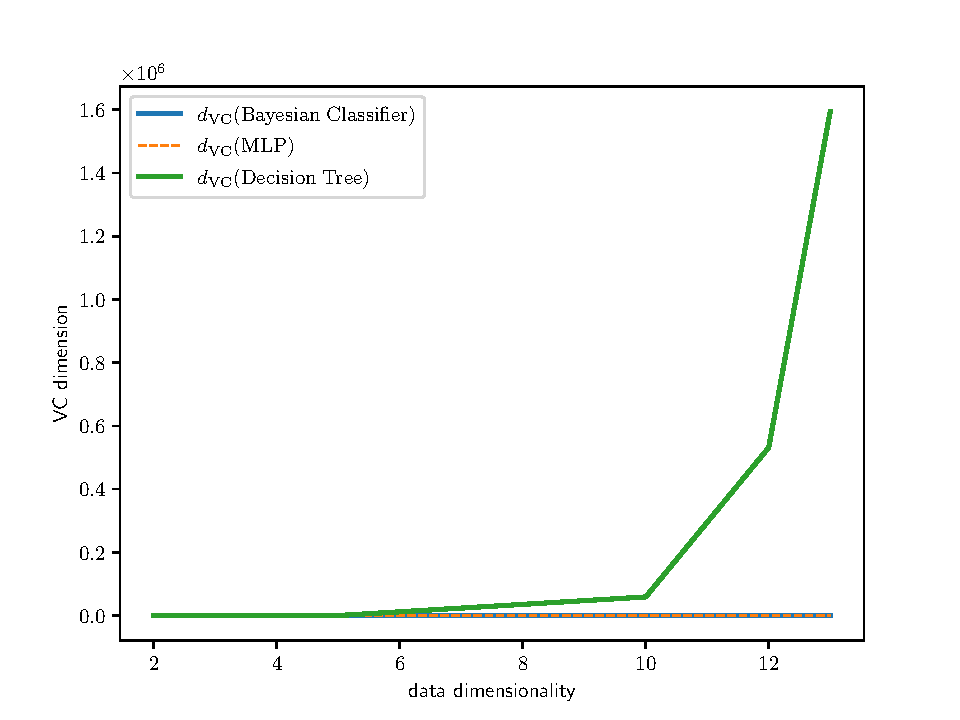
\includegraphics[scale = 0.75]{vc_4_a.pdf}
            \end{figure}
            In comparison to the other models, the VC dimension of the decision tree starts to explode exponentially for data dimensionalities as low as 12 (thus requiring exponentially larger datasets to mitigate overfitting risks).
            \vspace{1em}
            \item \quad 
            \vspace{-3.0em}
            \begin{figure}[H]
                \centering
                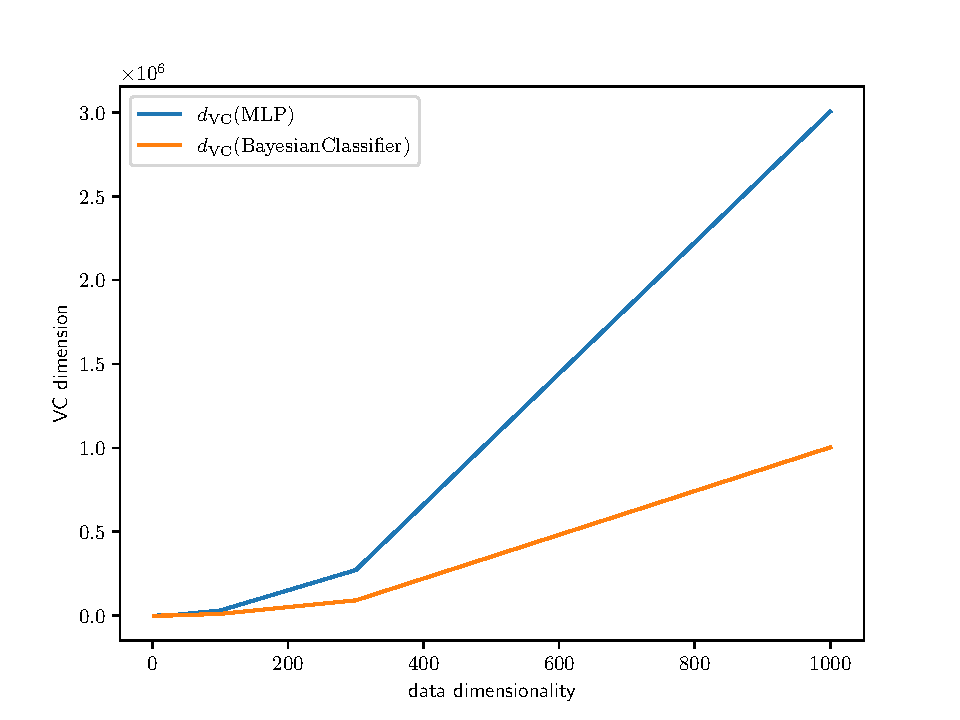
\includegraphics[scale = 0.75]{vc_4_b.pdf}
            \end{figure}
            We estimate that $d_{\text{VC}}(\text{MLP}) > d_{\text{VC}}(\text{Bayesian Classifier})$, with these values only diverging for $m \ge 300$ (albeit by not more than a multiplying constant, given their similar asymptotic behaviour).
        \end{parts}
    \end{questions}
    \section{Programming and critical analysis}
    \begin{questions}
        \setcounter{question}{3}
        \item \quad
        \begin{parts}
            \vspace{-1.6em}
            \item The produced solution yielded an ECR value of 13.5 for 2-means and 6.67 for 3-means.
            \item The produced solution yielded a Silhouette value of 0.5968 for 2-means and 0.52454 for 3-means. 
        \end{parts}
        \item \quad
        \vspace{-1.2em}
        \begin{figure}[H]
            \centering
            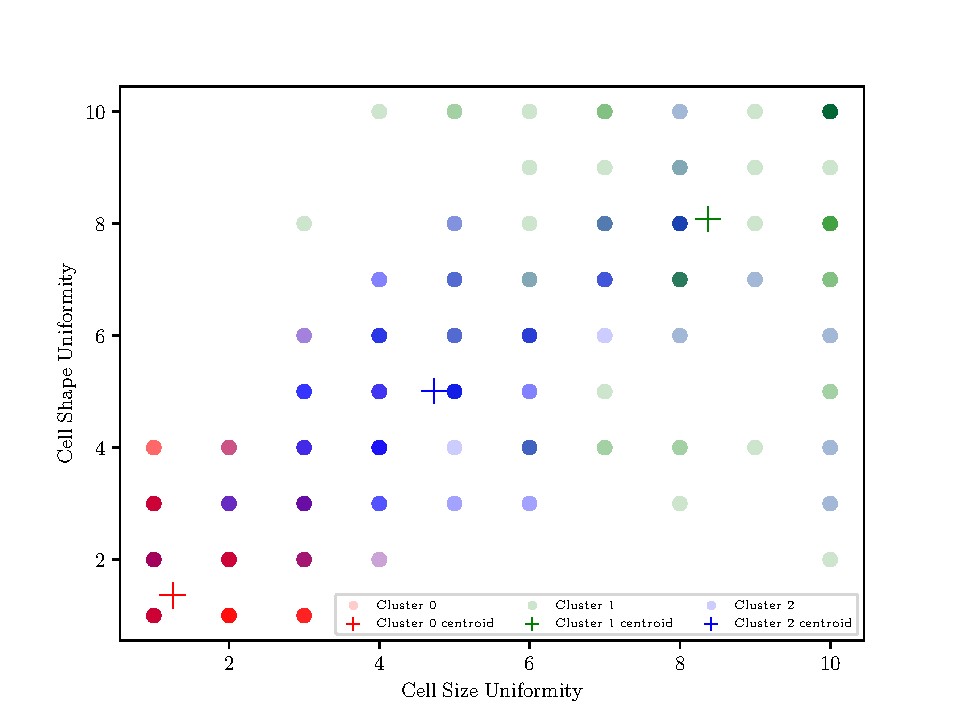
\includegraphics{3means.pdf}
        \end{figure}
        \item Assuming that the selected features are able to correctly capture the structure of the dataset, the plot above shows that the clustering solution yields poor separation, given the existence of instances with contiguous feature values that are assigned to different clusters. Furthermore, cohesion is also unsatisfactory: note the variance in cluster 1, which contains instances with feature values (4, 10) and (10, 2). This suboptimal performance can be explained by the fact that the dataset lacks circle-like concentrations of points that make the application of $k$-means suitable. Alternatively, the fact that $k$-means only considers Euclidean distances (and thus neglects feature importance) may make discerning cluster structures in this reduced input space not possible.
    \end{questions}

    \pagebreak
    \section{Appendix}
    \inputminted{python}{src/part02.py}
   
    
    
\end{document}